\chapter{Network CDNs}
\label{ch:ncdn}


The traditional tri-partite view of content delivery consists of three sets of entities: content providers (e.g., media companies, news channels, e-commerce sites, software distributors, enterprise portals, etc.), networks (e.g., telcos such as AT\&T, multi-system operators such as Comcast, and  ISPs), and content delivery networks (CDN) (e.g., Akamai, Limelight). 

Recent powerful trends are reshaping the simplified tripartite view of content delivery. A primary driver is the torrid growth of video \cite{nielsen-video-growth,cisco-videogrowth} and downloads traffic on the Internet. For example, a single, popular TV show with 50 million viewers, with each viewer watching an HD-quality stream of 10 Mbps, generates 500 Tbps of network traffic! The increasing migration of traditional media content to the Internet and the consequent challenges of scaling the network backbone to accommodate that traffic has necessitated the evolution of {\em network CDNs} (or \ncp s)\footnote{\ncp s are sometimes referred to as Telco CDNs, or Carrier CDNs. Further, they are referred to as a Licensed CDN when a pure-play CDN such as Edgecast\cite{edgecast} licenses the CDN software to a network to create an \ncp.} that vertically integrate CDN functionality such as content caching and redirection with traditional network operations \cite{hpcdn,telcowhitepaper,level3-cdn,att-cdn,verizon-cdn} (refer Figure \ref{fig:networkCDN}). A second economic driver of \ncp s is the desire of networks to further monetize the ``bits'' that flow on their infrastructure by contracting directly with content providers, or to offer value-added service packages to their own end-user subscribers  (e.g., Verizon's recent offering that delivers HBO's content to FIOS subscribers  \cite{fios}.


\begin{figure}
\centerline{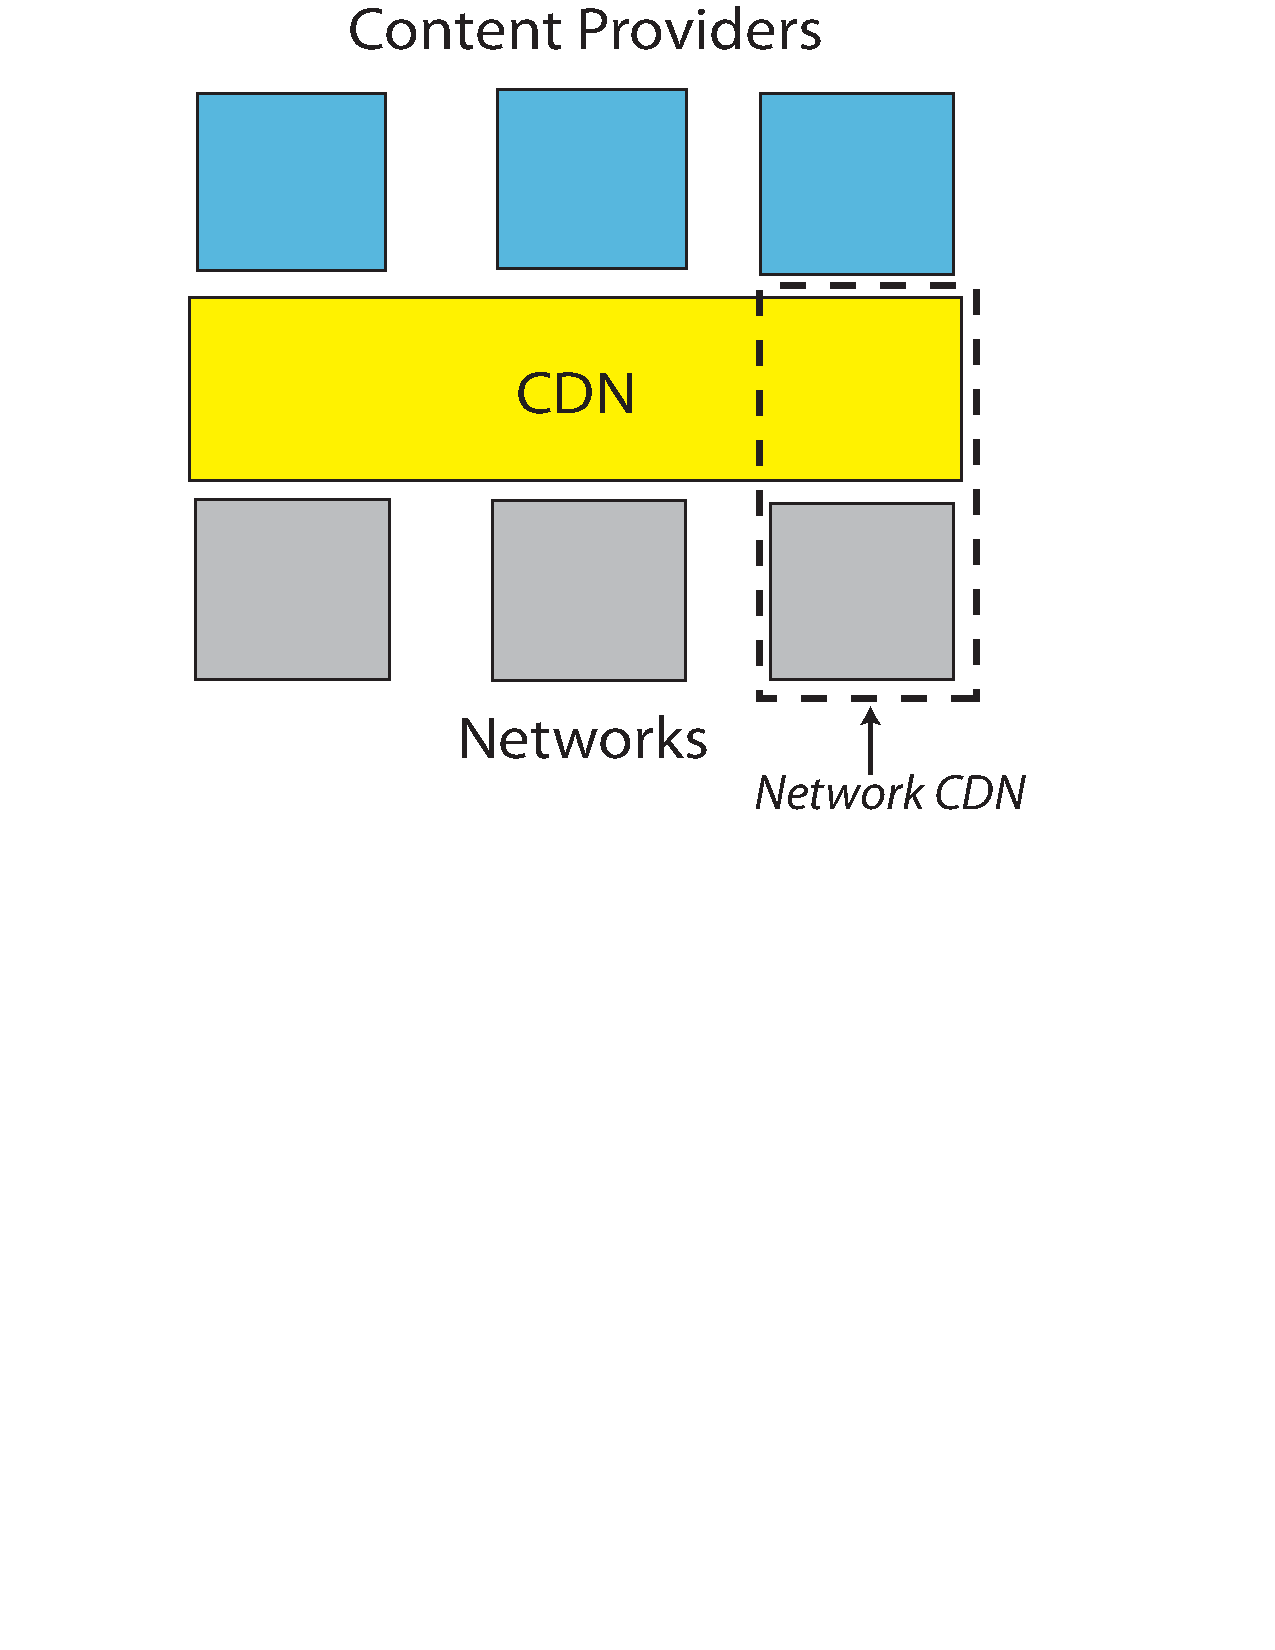
\includegraphics[height=2.5in]{ncdnpaper/NetworkCDN}}
\vspace*{-1.35in}
\caption{A tripartite view of content delivery.}
\vspace*{-0.25in}
\label{fig:networkCDN}
\end{figure}



As \ncp s control both the content delivery and network infrastructure, the costs and objectives of their interest are different both from a traditional CDN and a traditional ISP. In particular, an \ncp\ is in a powerful position to place content in a manner that ``shapes'' the traffic demand so as to optimize both network cost and user-perceived latency as illustrated using the example in Chapter \ref{ch:te-background}, Section \ref{sec:bg-ncdn}. Indeed, several recent works have alluded to the benefits of such joint optimization strategies in the context of cooperative or competitive interaction between ISPs and content providers \cite{P4P,JohariGameTheory,Jiang2009,catenew}. On the surface, an \ncp\ would appear to be the perfect setting for fielding joint optimization strategies as it eliminates potentially conflicting competitive interests. Nevertheless, \ncp s today continue to treat content delivery and traffic engineering concerns separately, operating the former simply as an overlay.

This disparity raises several research questions that form the focus of this chapter. How should an \ncp\ determine content placement, network routing, and request redirection decisions so as to optimize network cost and user-perceived latency? How much benefit do joint optimization strategies yield over simpler strategies as practiced today, and does the benefit warrant the added complexity?  How do content demand patterns and placement strategies impact network cost?  How do \planned\ strategies (i.e., using knowledge of recently observed demand patterns or hints about anticipated future demands) for placement and routing compare against simpler, \unplanned\ strategies?

Our primary contribution is to empirically analyze the above questions for realistic content demand workloads and ISP topologies. To this end, we collect content request traces from Akamai, the world's largest CDN today. We focus specifically on on-demand video and large-file downloads traffic as they are two categories that dominate overall CDN traffic and are significantly influenced by content placement strategies. Our combined traces consist of a total of 28.2  million requests from 7.79 million unique users who downloaded a total of 1455 Terabytes of content across the US over multiple days. Our main finding based on trace-driven experiments using these logs and realistic ISP topologies is that {\em simple, unplanned strategies for placement, routing, and redirection of NCDN content are better than sophisticated joint-optimization approaches}. Specifically,
\begin{itemize}
\item For NCDN traffic, simple \unplanned\ schemes for placement and routing (such as least-recently-used and InverseCap)  yield significantly lower (2.2--17$\times$) network cost and user-perceived latency than a joint-optimal scheme with knowledge of the previous day's demand\footnote{We use the term ``optimal'' when placement or routing is the solution of an optimization problem, but the solution may not have the lowest cost (for reasons detailed in Section \ref{sec:videodownload})}. 
\item NCDN traffic demand can be ``shaped'' by simple placement strategies so that  traffic engineering, i.e., optimizing routes with knowledge of recent traffic matrices, hardly improves network cost or user-perceived latency over \unplanned\ routing (InvCap).
\item For NCDN traffic, unplanned placement and routing is just 1\%-18\% sub-optimal compared to a joint-optimal placement and routing with perfect knowledge of the next day's demand at modest storage ratios ($\approx4$). % with simple optimizations such as content chunking and link-utilization-aware redirection.
\item With a mix of NCDN and transit traffic, traffic engineering does lower network cost (consistent with previous studies), but the value of traffic engineering substantially diminishes as the relative volume of NCDN traffic begins to dominate that of transit traffic.
\end{itemize}
\vspace{-0.08in}
%\item Future knowledge helps, i.e., demand-oblivious placement and routing is moderately worse compared to a joint-optimal placement and routing with perfect knowledge of the next day's demand at small to moderate storage ratios (<  2.2), but the difference reduces to less than 20\% at higher storage ratios  ($\approx$ 4). 

%\item Demand-oblivious placement and routing performs within 20\% of joint-optimal placement and routing with perfect knowledge of the next day's demand at a moderate storage ratios (\approx 4). 

%\item Simple hybrid strategies (partly demand-aware and partly demand-oblivious) do not improve upon a completely demand-oblivious strategy; and optimizations such as chunking do not qualitatively change our findings.


In the rest of this chapter, we first overview the \ncp\ architecture highlighting why it changes traditional ISP and CDN concerns (Section \ref{sec:ncdn-background}). Next, we formalize algorithms that jointly optimize content placement and routing in an NCDN (Section \ref{sec:optimize}). We then describe how we collected real CDN traces (Section \ref{sec:dataset}) and evaluate our algorithms using these traces and real ISP topologies (Section \ref{sec:ncdn-eval}). 

% We provide background material on content-aware traffic engineering for NCDNs  (Section~\ref{sec:background}). We then provide algorithms for content-aware traffic engineering that perform content placement, request redirection, and traffic routing to minimize MLU (Section~\ref{sec:optimize}).  Next, we evaluate our algorithms using extensive real-world traces from a large commercial CDN (Section~\ref{sec:empirical}). Finally, we present related work (Section~\ref{sec:related}) and conclusions (Section~\ref{sec:conclusions}).

%While traditionally networks lacked a direct relationship with content providers to deliver their content, the NCDN approach provides an avenue for networks to tap into that revenue stream. In addition, deploying an NCDN provides the additional benefit of higher performance for their subscribers that could form the basis for new differentiated services. As an example of this trend, consider the recent offering by Verizon that delivers HBO's content to FIOS TV subscribers

%Recent powerful trends are reshaping the simplified tripartite view of content delivery. A primary driver is the torrid growth of video and download traffic on the Internet.  Consider that a single major television show with a viewership of 50 million with each viewer watching a HD-quality stream of 10 Mbps generates 500 Tbps of network traffic! As traditional media such as television and movies migrate on to the Internet, the scaling of the network backbone to accommodate that traffic is a major technological challenge. This has necessitated the evolution of the {\em Network CDN\/} (NCDN, for short) that vertically integrates CDN functionality that provide scalability such as request  redirection and content caching with traditional network operations (See Figure~\ref{fig:networkCDN}).  A second economic driver for NCDNs is the desire of networks to monetize the ``bits'' that flow on their infrastructure. While traditionally networks lacked a direct relationship with content providers to deliver their content, the NCDN approach provides an avenue for networks to tap into that revenue stream. In addition, deploying an NCDN provides the additional benefit of higher performance for their subscribers that could form the basis for new differentiated services. As an example of this trend, consider the recent offering by Verizon that delivers HBO's content to FIOS TV subscribers.

%The mechanism for constructing an NCDN may vary from a complete turnkey solution where a traditional CDN deploys their service at the network's PoPs, to a software licensing solution where a traditional CDN licenses their software for the network to use, to the network building the CDN functionality themselves. 
%Independent of the mechanism, 

%NCDNs raise important scientific questions on how content delivery functionality impacts the traditional traffic engineering focus of networks.  While the two functionalities are performed separately today,  the trend towards NCDNs opens up for the first time the possibility of jointly optimizing content delivery and traffic engineering, as both are now controlled by the same business entity. To our knowledge, our work is the first to examine the rich possibilities that are opened up by this nexus.  {\em A primary contribution of this paper is that effective content delivery can simplify or even completely obviate the need for complex traffic engineering implemented by networks today. } 

%{\bf NCDN Architecture.} 
\begin{figure}
\vspace*{-0.7in}
\centerline{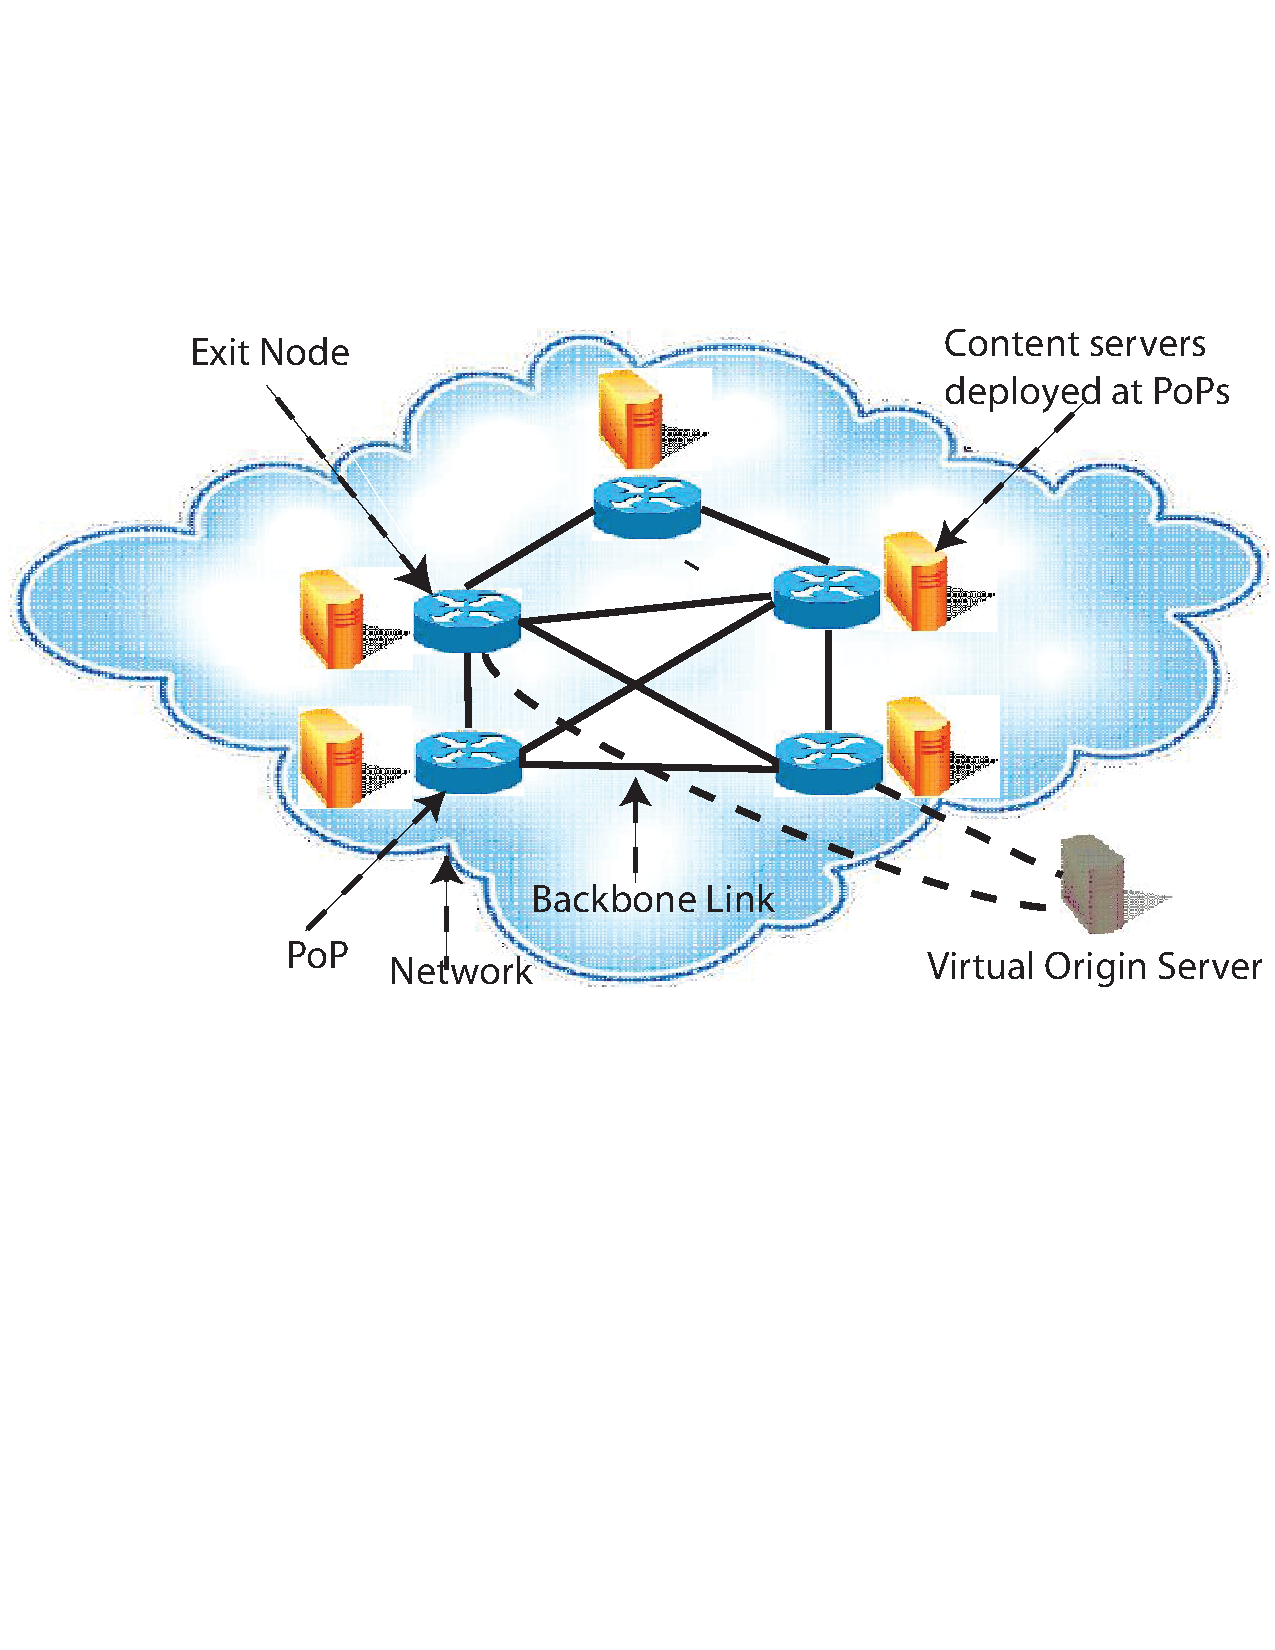
\includegraphics[height=3.5in]{ncdnpaper/NCDNArch}}
\vspace*{-1.3in}
\caption{NCDN Architecture}
\label{fig:NCDNArch}
\end{figure}
%A typical NCDN architecture follows closely the architecture\footnote{For a detailed treatment of the architectural components of a global CDN, the reader is referred to \cite{akamai-overview}.} of a global CDN, except that the content servers are deployed at PoP's within the network rather than globally across the Internet (See Figure~\ref{fig:NCDNArch}).   Further, an NCDN typically serves content only to downstream end-users and subscribers of the network, rather than to a global audience. Each content provider publishes all their content to {\em origin servers} that they maintain. The origin servers may be mirrored across different data centers on the Internet and these mirrors could be hosted external to the NCDN itself on a different network. 

%Each PoP is associated with the set of end-users downstream from it who request content, such as requests for web content, downloads, and video content. Thus each PoP can be viewed as a source of demand for content that must be satisfied either by the content servers local to the PoP,  or by downloading from a  content server at a different PoP, or by downloading the content directly from the origin. When an end-user requests a piece of content,  the request is first routed to the content servers deployed at the PoP to which the end-user is connected.  If a content server at that PoP has the requested content in their cache, it serves that content to the end-user. Otherwise, if the requested content is cached at another PoP in the network, the content is downloaded from that PoP and served to the end-user. Finally, if the content is not present in any content server in the network, it is downloaded directly from the origin servers of the content provider. 

%{\bf content delivery.}  The two key aspects of content delivery that we study are {\em content placement} that determines which piece of content is placed on content servers of which PoP (potentially with replication) and {\em request redirection\/} that determines which content servers are used to serve each requested piece of content.  Note that when a piece of requested content is present in content servers at multiple PoPs, the request redirection policy determines which PoP serves the request. 

%{\bf Traffic Engineering.} A key component of network operations is routing the traffic demands on the backbone network so as to enhance network performance and maximize the utilization of network resources \cite{fortz2002traffic}. More formally, given the topology of the network with link capacities and a demand matrix $D$ that specifies the traffic flow that must be routed between each pair of nodes (i.e., PoPs) $(s, t)$,  the goal of traffic engineering is to determine the path(s)  to route each such traffic flow such that a predetermined objective function is minimized\cite{fortz2000internet}.  The most common objective function is to minimize the maximum link utilization (MLU) in the network, where link utilization is the ratio of the traffic flow on that link and its capacity. The paths to route the traffic flows in the network are themselves constrained by the intra-domain routing protocol impmemented by the network. The protocol that is most widely used in practice is Open Shortest Path First (OSPF) where the network operator assigns weights to each link and the path used between $s$ and $t$ is simply the shortest path(s) between the nodes using the weights as the lengths of the links. Further, if a node has multiple outgoing links that each yield the same distance to the destination, traffic is split evenly between those links. A simple special case of OSPF that is commonly used is InverseCapacity routing (InvCap) where the OSPF weight of each link is statically set to be the inverse of its capacity.  More flexible than OSPF is the Multi-protocol Label Switching (MPLS) protocol. MPLS can implement any set of routing paths, since in principle the route of each packet can be specified in an independent fashion. However,  MPLS is more complex to implement compared to OSPF variants. Our critical observation is that effective content delivery can ``shape'' the traffic demand matrix $D$ in manner that simplifies or even obviates the need for complex traffic engineering.

%{\bf Our Contributions.} Need to write.

%{\bf Roadmap.} We provide background material on content-aware traffic engineering for NCDNs  (Section~\ref{sec:background}). We then provide algorithms for content-aware traffic engineering that perform content placement, request redirection, and traffic routing to minimize MLU (Section~\ref{sec:optimize}).  Next, we evaluate our algorithms using extensive real-world traces from a large commercial CDN (Section~\ref{sec:empirical}). Finally, we present related work (Section~\ref{sec:related}) and conclusions (Section~\ref{sec:conclusions}).

%The boundary between the entities which route traffic, i.e., Internet %service providers (ISPs), and the entities which publish content is %increasingly blurring in today's Internet with one progressively taking %the role of another. For example, top ISPs such as AT\&T, Level-3  and %Verizon  are also among the top content distributors and top content %distributors such as Comcast and manage their own networks. 

%We envision a network where the owner termed as \textbf{N}etwork and %\textbf{C}ontent \textbf{P}rovider (\textbf{\ncp})  can decide the %placement of content  at nodes in the network, in addition to choosing %the routes between nodes, as is done today.  Each user in the network %termed as \textbf{C}ontent \textbf{C}onsumer (\textbf{\cc}) can demand %any content provided by its \ncp.

%Since an \ncp\ manages network as well as content served through the network, it needs to solve problems faced by ISPs which manage traffic in their networks , as well as CDNs, which manage content from their clients. For example, where to place content? How many copies  of each content to place ? How to  determine routes  between nodes while keeping network links free from congestion ? How to load balance among servers at different PoPs?
%How to load balance between sets of servers across nodes?


%The task for an \ncp\ can be broken down into two sub-problems: (1) Network and storage capacity planning over a long term (2)  Managing content storage and network traffic on a day-to-day basis. In this work, our focus is the later problem. But we also study the effect of network and storage capacity available in the network on our results.


%There are three metrics of interest for an \ncp:  (1) Congestion of links in the network (2) 	Load on the servers at each PoP (3) Link latency between \cc's and content they are accessing.  An \ncp's strategy for content placement and routing affects all three metrics mentioned above. For example, replicating a very popular content at many locations in the network will reduce congestion, will distribute the load from servers at one PoP to multiple PoPs and  reduce the latency between \cc's and the content. 

%In this context, our work is motivated by the question: ``Which among content placement and routing plays a greater role in optimizing the metrics of interest for an \ncp?" We compare the performance of simple vs. sophisticated strategies for routing and for deciding content placement. 

%Based on our experiments using  traffic data from three ISPs, we conclude that optimizing content placement is considerably more important  than optimizing routing for an \ncp. A strategy which decides  content placement optimally while adopting a simple static routing performs much better than a strategy which uses a simple content placement with  an optimal routing; it even performs nearly identical to a strategy which makes both content placement and routing decisions optimally. 


%Our paper makes the following contributions:

%\begin{itemize}
%\item
%A  comparison of content placement strategies in terms of their network cost based on real world traces from a very large CDN including three major sources of Internet traffic - short video, long video and software downloads.
%\item
%hypothetical: A combination of static and dynamic placement strategies performs best or equally best for all three traces. Using a dynamic placement alone performs close to optimal for short videos, but is sub-optimal for other content types. Using a purely static placement strategy 
%\item
%hypothetical: Using the best content placement strategy along with a naive routing reduces network cost more than optimizing routing but using a significantly worse content placement strategy.
%\end{itemize}


%\ncp's  solution to these questions must consider the performance for users in the network, as well as cost incurred by \ncp.  From an \ncp's perspective the objective would be to minimize the capital expenditure cost  of storage and  links, assuming that operational cost does not rise on decreasing capital expenditure. From a \cc's perspective, the performance improves on reducing the delay between \cc\ and the node that is storing the content it is consuming.
%
%
%We split the network management problem for an \ncp\ into three problems: (1) which location/s is each content placed ? (2) which replicas for a content are used for  \cc's at a node ? (3) how is traffic routed between two locations ? 

 
% content management + network management 

%We take the first step towards designing a network management solution for the NCP by comparison four design choices for an 




%ISPs change routing in the network in response to changing traffic demands in order to reduce the congestion in the network. This process is called traffic engineering. Specifically, ISPs optimize the maximum link utilization metric (MLU) so as to reduce the link utilization of backbone links in the network which in turn is expected to minimize congestion. Traffic engineering is widely used by ISPs today and techniques for traffic engineering have seen a large body of work in the research community.

%If an ISP can place the content being distributed in the network, it can minimize congestion also by changing the content placement. Optimizing content placement includes deciding how many replica of each content to store in the network, where to place content in the network, and how to split traffic demand among multiple servers in the network. Changing content placement can modify the traffic on links in the network and therefore optimizing placement and help reduce MLU in the network. In particular, creating additional replicas can significantly reduce the traffic in the network since  content can be obtained from nearby locations. If a content is placed at the PoP which is requesting the content, the traffic demand for the content from that node vanishes. 

%Assuming that an ISP could optimize both content placement and routing, what should an ISP  optimize for traffic engineering.  To this end we compare traffic engineering schemes which belong to one of the following four categories: 
%(1) Simple Routing + Simple Placement: 
%(2) Optimal Routing + Simple Placement
%(3) Simple Routing + Optimal Placement
%(4) Optimal Routing + Optimal Placement

%We present linear programs to compute routing and placement for these traffic engineering schemes. Using two sets of ISP topologies and traffic matrices, we compare the performance of the above TE schemes.

%Our main conclusions from this work are as follows:
%\begin{enumerate}
%\item 
%Optimal Placement with a InvCap routing scheme (InvCapOptimalPlacement)  performs identical to the joint optimal solution of MLU and routing.
%\item
%Optimal routing coupled with a simple placement strategy performs sub-optimally compared to optimizing both placement and routing.
%\item
%Optimizing placement for content with local popularity gives up to a 10$\times$ reduction in MLU compared to other TE schemes.
%\end{enumerate}




%An ISP network where ISP is both the content distributor and the network service provider. In this case, ISP can optimize both routing as well as the content placement. We assume that the content placement allows a small degree of replication in the network, which provides location diversity for content in the network. An ISP seeks to maximize the traffic demand which can be served through its network. Therefore it optimizes MLU. 

%\textbf{hypothesis: placement benefits MLU more than routing}

%Our hypothesis is that placement is more important than routing to maximize the maximum served traffic demand in the network, that is optimal placement is more valuable than optimal routing. 

%\textbf{problem: How much replication is needed for optimal placement to perform close to optimal (placement + routing) ?}

%If this is indeed the case, then ISP can place content optimally in the network and perform a simple routing such as InvCap in the network.  Building up on our previous results, this would suggest that ISPs do not need to do any traffic engineering in the network. The next important question is that how much location diversity is needed to gain the benefits of optimal placement over optimal routing ?

%\textbf{problem: Which algorithm to use for placement?}
%
%- Optimal
%
%- Heuristic ?
%
%\textbf{problem: at what timescales can we compute placement ?}
%
%- 
%
%\textbf{conclusion: ?}
%
%just placement is good enough to get close to (optimal placement + optimal routing).
%
%
%2. Examples/results motivating optimal placement over routing
%
%3. Network model and algorithms
%
%3.1 Network model
%
%3.2 Joint Placement + Routing  : 
%
%- NP Hard
%
%- Linear program for this problem
%
%- Rounding techniques
%
%3.3 Fixed routing + Optimal Placement 
%
%- NP Hard 
%
%- Changes to Linear program
%
%- Rounding techniques
%
%3.4 Simple Placement Strategies
%
%
%
%4. Evaluation
%
%- file popularity distribution : zipf-like, homogenous
%
%- file size : s
%
%4.1 Effect of file popularity distribution across nodes
%
%- homogenous : gravity
%
%- heterogenous : gravity
%
%- mix of homo and hetero
%
%4.2 Effect of traffic demand
%
%- gravity
%
%- 
%
%5. Related work
%
%6. Conclusion



%\textbf{Previous Intro}
%
%The goal of the project is to develop algorithms for traffic engineering when the ISP can place content as well route traffic. This problem can be divided into two sub problems: (1) placing  content optimally in the network  (2)  routing optimally when the content location as well as the traffic demand in the network is known.
%
%To our knowledge, the first question, i.e., optimally placing content to optimize a traffic engineering metric has not been analyzed in previous work. The solution to the second problem can be obtained using linear programs which are described in Section \ref{sec:linearprograms}.
%
%Problems:
%
%1. For a set of traffic demands from a set of sink nodes, optimize routing when (1) there is only one type of content (2) there are multiple types of content. Vary the number of locations.
%
%2. For a set of traffic demands from a set of sink nodes, optimize C = w * COST(content placement)/OPTCOST + (1- w) * MLU(routing)/OPTMLU
%

%
%Sequence of steps for optimal MLU:
%
%\begin{enumerate}
%\item
%Show that finding the optimal placement problem to optimize MLU is NP-hard.
%\item
%Compare the performance of heuristic algorithms for different levels of diversity: Random, probabilistic rounding, local search.
%\item
%Compare the performance of heuristic algorithms when there are different types of content.
%\end{enumerate}


%\section{Background}
%
%\subsection{Changing Internet}
%
%\subsection{Multiple ways to engineer traffic}
%
%\subsection{Challenges}


%An important criterion in designing a network management scheme is how often can we change the network configuration: The placement can only be changed in the order of days since it incurs a huge overhead in terms of time and network bandwidth to change the content placement. The flow splits among multiple locations and the routing can be changed in the order of minutes or hours since they only require changing few parameters in the network, the resulting change can be quickly realized. Therefore, we assume that a placement operation runs on a slower time scale than computing routing or changing flow splits in the network.

%Flow splits among multiple locations can be done in multiple ways for the same placement of content. But, we combine actions (1) and (2) into one action. This implies (1) and (2) are (1) and (2) happen together in the network and at a slower time scale than changing the routing in the network.

